% Q6: schematic cosine graph with the source's labelled intercept and maximum.
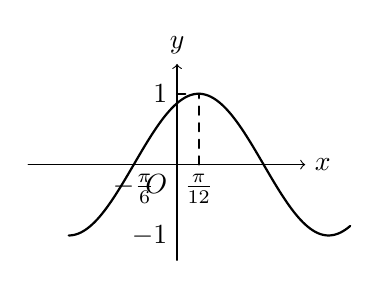
\begin{tikzpicture}[line cap=round,line join=round,x=1.05cm,y=0.9cm]
  \draw[->] (-1.8,0)--(1.55,0) node[right] {$x$};
  \draw[->] (0,-1.35)--(0,1.42) node[above] {$y$};
  \draw[thick,dashed] ({pi/12},0)--({pi/12},1);
  \draw[thick,dashed] (0,1)--({pi/12},1);
  \draw[thick,domain=-75:120,samples=120,variable=\t]
    plot ({\t*pi/180},{cos(2*\t-30)});
  \node[below left] at (0,0) {$O$};
  \node[left] at (0,1) {$1$};
  \node[left] at (0,-1) {$-1$};
  \node[below] at ({-pi/6},0) {$-\frac{\pi}{6}$};
  \node[below] at ({pi/12},0) {$\frac{\pi}{12}$};
\end{tikzpicture}
